\documentclass[envcountsect,aspectratio=169]{beamer}
\usepackage{etex}
\usefonttheme[onlymath]{serif}
\usepackage[utf8x]{inputenc}
\usepackage[brazilian]{babel}
\usepackage{amsthm,amssymb}
%\usepackage{graphicx}
\usepackage{wrapfig}
\usepackage[]{qrcode}
\usepackage{color}

\usepackage{multicol}
\usepackage{makecell}
\usepackage{syntonly}
\hypersetup{colorlinks,linkcolor=,urlcolor=blue}


\usepackage{pgf,tikz}
\usetikzlibrary{calc}
\usetikzlibrary{positioning}
\usetikzlibrary{decorations.pathreplacing}
\usepackage{tkz-euclide}

%---------------- tabu package 
\usepackage{xcolor}
\usepackage{colortbl}
\usepackage{tabu}

%--------------------------------
\usepackage[labelformat=empty]{caption}
\setbeamertemplate{caption}[numbered]{}

\usetheme{Madrid}
\usecolortheme{beaver}


\setbeamertemplate{theorems}[numbered]
\setbeamertemplate{enumerate items}[circle]
\newtheorem{nada}{Nada}


\theoremstyle{definition}
\newtheorem{defin}[nada]{Defini\c c\~ao}
\newtheorem{prop}[nada]{Proposi\c c\~ao}

\newtheorem{corol}[nada]{Corol\'ario}

\newtheorem{teo}[nada]{Teorema}

\newtheorem{lema}[nada]{Lema}



\newtheorem{outline}{\timesbold outline rem proof}

\newtheorem{obs}[nada]{Observação}
\newtheorem{afir}{Afirmação}

\makeatletter
\def\th@exercicio{%
	\normalfont % body font
	\def\inserttheoremblockenv{alertblock}  
}
\theoremstyle{exercicio}
\newtheorem*{exer}{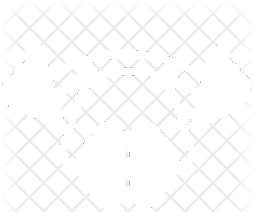
\includegraphics[scale=0.06]{w-brainb.png} Exercício}
\makeatother

\newtheorem{casa}{
\includegraphics[scale=0.035]{w-homework.png} Para Casa}
\makeatother




\makeatletter
\def\th@something{%
	\normalfont % body font
	\def\inserttheoremblockenv{exampleblock}  
}
\theoremstyle{something}
\newtheorem*{exe}{
\includegraphics[scale=0.3]{exemplo.png} Exemplo }
\makeatother

%\setbeamercolor{block title}{bg=cyan, fg=white}

\newtheorem*{casa-comp}{
\includegraphics[scale=0.035]{w-homework-comp.png} Tarefa Computacional}
\makeatother

\makeatletter
\def\th@resp{%
	\normalfont % body font
	\def\inserttheoremblockenv{block}  
}
\theoremstyle{resp}
\newtheorem*{resp}{\includegraphics[scale=0.01]{White_check.png} Resposta}
\makeatother


\makeatletter
\def\th@desafio{%
	\normalfont % body font
	\def\inserttheoremblockenv{alertblock}  
}

\theoremstyle{desafio}
\newtheorem*{desafio}{\includegraphics[scale=0.02]{desafio-branco.png} Desafio}
\makeatother


%%%%%%%%%%%%%%%%%%%%%%%%%%%%%%%%%%%%%%%%%%%%%%%%%%%%%%%%%%%%%%%%%%%%%%%%%%%%%%%%%%%%%%%

\newcommand{\cqd}{\hfill \framebox[7pt]{} \mbox{} \medskip}
\newcommand{\R}{\mathbb{R}}
\newcommand{\xo}{{\color{blue}x_0}}
\newcommand{\id}{\operatorname{I}}
\newcommand{\rA}{{\color{red}A}}
\newcommand{\raa}{{\color{red}a}}
\newcommand{\Xo}{{\color{blue}X_0}}
\newcommand{\rT}{{\color{red}T}}
\newcommand{\xxo}{{\color{blue}\mathbf{x_0}}}
\newcommand{\dt}[1]{{\color{blue}#1}}
%%%%%%%%%%%%%%%%%%%%%%%%%%%%%%%%%%%%%%%%%%%%%%%%%%%%%%%%%%%%%%%%%%%%%%%%%%%%%%%%%%%%%%%


\begin{document}

%\setbeamercovered{transparent}
\title[Minicurso sobre EDOs em Espaços de Banach]{Minicurso EDOs em Espaços de Banach}
\author[Luiz Viana/Reginaldo Demarque]{
\vspace{-.5cm}
\begin{equation*}
{\normalsize {\color{blue} 
\begin{cases}
x'(t)={\color{red}A}x+{\color{black}f},& t\in [0,+\infty)\\
x(0)=x_0
\end{cases}}
}
\end{equation*}
\begin{equation*}
{\footnotesize {\color{blue} 
x(t)=e^{t\color{red}A}x_0+\int_0^t e^{(t-s)\color{red}A}{\color{black}f(s)}ds}
}
\end{equation*}\\
Prof. Luiz Viana e Prof. Reginaldo Demarque}

%%%%%%%%%%%%%%%%%%%%%%%%%%%%%%%%%%%%%%%%%%%%%%%%%%%%%%%%%%%%%%%%%%%%%%%%%%%%

\logo{
\includegraphics[scale=0.05]{UFF_brasao.png}}

\institute[IMEUFF]{Universidade Federal Fluminense\\
Instituto de Matemática e Estatística \\
Programa de Pós-Graduação em Matemática \\
}
\date{{\color{orange} 12 à 21 de fevereiro de 2025}}

\frame{\titlepage}
%%%%%%%%%%%%%%%%%%%%%%%%%% sumario  %%%%%%%%%%%%%%%%%%%%%%%%%%%%%%%%

\frame{
 \frametitle{Sumário}
 \tableofcontents
}

\AtBeginSection[]
{
 \begin{frame}

  \frametitle{Sumário}
  \tableofcontents[currentsection]

 \end{frame}
}
\section{Apresentação}

\begin{frame}{Apresentação do Minicurso}

\begin{itemize}


\item \textbf{Ementa}:  Definição de Espaços de Banach. Exponencial de Operadores Lineares Limitados. Semigrupos de classe $C^0$.  Gerador Infinitesimal. Existência e Unicidade para o PVI. Resolvente de um operador. Semigrupos das Contrações. O Teorema de Hille-Yosida. Aplicações e perspectivas de pesquisa.

\item \textbf{Material}: \href{https://reginaldodr.github.io/academic/semigrupos/minicurso-2025-verao.html}{reginaldodr.github.io/academic/semigrupos/minicurso-2025-verao}

\begin{center}
\qrcode[hyperlink,height=1in]{https://reginaldodr.github.io/academic/semigrupos/minicurso-2025-verao}
\end{center}
\end{itemize}

\end{frame}
\section{Bibliografia}

\begin{frame}\frametitle{Bibliografia}
%\begin{scriptsize}

\begin{thebibliography}{}
\beamertemplatebookbibitems
\bibitem[Alvercio, 2011]{alvercio}
Alvércio Moreira Gomes
\newblock {\em  Semigrupos de Operadores Lineares e Aplicações às Equações de Evolução}
\newblock Editora UFRJ, 2ª ed., Rio de Janeiro, 2005.
\newblock \href{https://www.im.ufrj.br/index.php/pt/estrutura/editora-im/matematica/1931-semigrupos-de-operadores-lineares-e-aplicacoes-as-equacoes-de-evolucao}{Edição digital disponibilizada aqui}

\bibitem[Kesavan, 2015]{kesavan}
S. Kesavan
\newblock {\em  Topics in Functional Analysis and Applications}
\newblock New Age International Ltd, 2ª ed., New Delhi, 2015.

\end{thebibliography}

\end{frame}



\section{Prelimiares}

\subsection*{Espaços Normados}

\begin{frame}{Espaços Normados}
\begin{defin}
    Uma {\color{blue} norma} é
\end{defin}
\end{frame}

\subsection*{Operadores Lineares Ilimitados}

\begin{frame}{Operadores Lineares ilimitados}
Sejam $X$ e $Y$ dois espaços de Banach. Seja $A:D(A)\subset X\longrightarrow Y$ um operador linear,  onde $D(A)$ é um subespaço de $X$, chamado de {\color{blue} domínio} de $A$.
\medskip
Dizemos que $A$ é {\color{blue}limitado (ou contínuo)} se $D(A)=X$ e se existe  $C>0$ tal que 
\begin{equation}\label{ltdo}
\|Ax\|_{Y}\leq C\|x\|_X, \ \forall x\in D(A).
\end{equation}
Denotaremos por $\mathcal{L}(X,Y)$ o espaço de Banach dos {\color{blue} operadores lineares limitados} com norma dada por
\[\|A\|_{_{\mathcal{L}(X,Y)}}=\sup\limits_{x\in X, x\neq 0}\frac{\|Ax\|_{_Y}}{\|x\|_{_X}},\]
por $\mathcal{L}(X)=\mathcal{L}(X,X)$ e $X'=\mathcal{L}(X,\R)$.
$A$ é dito ser {\color{blue}ilimitado} quando não satisfaz \eqref{ltdo}. Dizemos que $A$ é {\color{blue}densamente definito} se $\overline{D(A)}=X$.
\end{frame}

\begin{frame}{ }
\begin{exe}

\end{exe}
\begin{exer}
Se $A,B\in \mathcal{L}(X)$ mostre que $A\cdot B\in \mathcal{L}(X)$ e 
\[{\color{red}\|A\cdot B\|_{_{\mathcal{L}(X)}}\leq \|A\|_{_{\mathcal{L}(X)}}\|B\|_{_{\mathcal{L}(X)}} }\]
\end{exer}
\end{frame}

\begin{frame}{}
 Seja    
\end{frame}


\subsection*{Integral Vetorial}

\begin{frame}{Integral Vetorial}
\begin{defin}
Sejam $X$ um espaço de Banach e $u:[a,b]\longrightarrow X$ uma aplicação tal que, para cada $\varphi\in X'$,  a função real
\[t\in [a,b] \longmapsto \langle\varphi, u(t) \rangle_{X'X}\in \R,\]
seja integrável. Dizemos que $u$ é integrável se existe {\color{blue} um vetor $v\in X$} que satisfaz:
\[\langle \varphi, v\rangle_{X',X}=\int_a^b \langle\varphi, u(t) \rangle_{X'X}\,dt,\ \forall \varphi\in X'.\]
Em caso afirmativo, $v$ é único e escrevemos
\[v=\int_a^b u(t)\,dt.\]

\end{defin}
\end{frame}

\begin{frame}{ }
\begin{prop}
Se $u:[a,b]\longrightarrow X$ é {\color{blue}contínua}, então $u$ é integrável. Além disso, 
\begin{enumerate}
    \item $\displaystyle\left\|\int_a^b u(t)\,dt\right\|\leq \int_a^b \|u(t)\|\,dt$
    \item Se $A\in \mathcal{L}(X,Y)$, então
    \[ A\left(\int_a^b u(t)\,dt\right)=\int_a^b A(u(t))\,dt. \]
\end{enumerate}

\end{prop}
\end{frame}

\section{Exponencial}

\begin{frame}{A função exponecial}
A função {\color{blue}logaritmo natural} é a bijeção contínua (com inversa contínua), definida por
\[
\displaystyle \log : x\in (0,+\infty ) \longmapsto \int_{1}^{x}\frac{1}{t}\,dt  \in \mathbb \R.
\]

A inversa de $\log :(0,+\infty ) \longrightarrow \mathbb R$ é a função exponencial $\exp :\mathbb R \longrightarrow (0,+\infty)$, e usualmente escrevemos 
\[
\displaystyle e^{x} :=\exp(x) \text{  para cada } x\in \mathbb R.
\]
Cabe recordar que:
\begin{itemize}
\item $e^{0}=1$;
\item $e^{x+y} = e^x \cdot e^{y}$ para quaisquer $x,y\in \mathbb R$;
\item $(e^x)' = e^x$ para todo $x\in \mathbb R$. 
\end{itemize}
\end{frame}


\begin{frame}{Solução do PVI}
Dados ${\color{red}a}\in \mathbb R$ e ${\color{blue}x_0} \in \mathbb R$, podemos constatar que a única função $x:[0,+\infty) \longrightarrow \mathbb R$ solução do \textbf{problema de valor inicial}
\[
\begin{cases}
    x'(t)={\color{red}a}x,\ t\in [0,+\infty);\\
    x(0)={\color{blue}x_0},
\end{cases}
\]
é dada por $x(t)={\color{blue}x_0}e^{{\color{red}a}t}$.
\end{frame}

\begin{frame}{Propriedades das Soluções}
Denotando $x(t)=S(t){\color{blue}x_0}$, fazemos as seguintes considerações:
\begin{enumerate}[a]
\item Para cada $t\in \R$, 
\[
\displaystyle S(t):\hspace{-.5cm} \underbrace{\color{blue}x_0}_{\text{dado inicial}}
\hspace{-.5cm} \in \R \longmapsto \underbrace{S(t){\color{blue}x_0}}_{\text{Solução do PVI}}\hspace{-0.5cm} \in \R
\]
é uma {\color{blue}função linear}.

\item $S(0){\color{blue}x_0} = x(0)={\color{blue}x_0}$, para cada ${\color{blue}x_0}$ fixado em $\mathbb R$, ou seja, $S(0)$ é exatamente a função identidade $\id:x\in \R \longmapsto x\in \R$;

\item Fixados $t,s\in [0,+\infty)$ e $\xo \in \R$, temos
\begin{equation*}
\displaystyle S(t+s)\xo = S(t) S(s)\xo.
\end{equation*}
\end{enumerate}
\end{frame}

\begin{frame}{Sistema de Equações}
Dada uma matriz $\rA$ em $\mathcal M _{n\times n} (\mathbb R )$ considere o sistema de EDOs
\[
    X'(t)=\rA X,\ t\in [0,+\infty),
\]
isto é,
\[
\begin{bmatrix}
x_1'(t)\\ x_2'(t)\\ \vdots \\ x_n'(t)
\end{bmatrix}
={\color{red}\begin{bmatrix}
a_{11} & a_{13} & \cdots & a_{1n}\\
a_{21} & a_{23} & \cdots & a_{2n}\\
\vdots & \vdots & \ddots & \vdots\\
a_{n1} & a_{n3} & \cdots & a_{nn}
\end{bmatrix}}
\begin{bmatrix}
x_1(t)\\ x_2(t)\\ \vdots \\ x_n(t)
\end{bmatrix}
\]

\end{frame}


\begin{frame}{Sistema de Equações}
Dada uma matriz $\rA$ em $\mathcal M _{n\times n} (\mathbb R )$ considere o PVI
\[
\begin{cases}
    X'(t)=\rA X,\ t\in [0,+\infty);\\
    X(0)=\Xo \in \mathcal M_{n\times 1} (\R ),
\end{cases}
\]
A solução procurada é um caminho 
\[
X: [0,+\infty) \longrightarrow   \mathcal M _{n\times 1} (\R ).
\]
Em analogia ao caso unidimensional
\[
X(t)=e^{t\rA}\Xo 
\]
\end{frame}


\begin{frame}{Exponencial de Matrizes}
Recordemos que a norma em $\mathcal M_{n\times n} (\R)$ é dada por
\[
\|\rA\|=\bigg( \sum_{i,j=1}^{n} |\raa_{ij}|^2 \bigg)^{1/2}
\]
para cada $\rA=[\raa_{ij}]_{i,j=1}^{n} \in \mathcal M_{n\times n} (\R)$. 

\begin{definition}\label{expmatrix}
    Seja $\rA\in \mathcal M_{n\times n} (\R)$. A {\color{blue}exponencial de} $\rA$ é dada por
    \begin{equation}\label{exp}
    \displaystyle e^{\rA}:=\sum_{j=0}^{\infty} \frac{\rA^j}{j!}=\id + \rA + \frac{1}{2}\rA^2+\frac{1}{3!}\rA^3+\cdots+\frac{1}{n!}\rA^n+\cdots . 
    \end{equation}
\end{definition}
\end{frame}

\begin{frame}
  \begin{enumerate}[(a)]
 \item A série de matrizes, dada em \eqref{exp}, é 
{\color{blue}absolutamente convergente}, isto é,
    \[
    \displaystyle \sum_{j=0}^{\infty} \frac{\| \rA^j \|}{j!}
    \]
    é sempre uma série de números reais convergente.
    \item $S(t)\Xo := e^{t\rA} \Xo$ a única solução do problema de valor inicial
    \[
\begin{cases}
    X'(t)=\rA X,\ t\in [0,+\infty);\\
    X(0)=\Xo \in \mathcal M_{n\times 1} (\R ),
\end{cases}
\]
    \end{enumerate}
\end{frame}

\begin{frame}

\begin{enumerate}[c]
    \item A aplicação $S(t): \mathcal M_{n\times 1} (\R) \longrightarrow \mathcal{M}_{n\times 1} (\R)$ possui propriedades análogas àquelas obtidas no caso unidimensional. Mais precisamente,
    \begin{itemize}
    \item Para cada $t\in [0,+\infty)$, $S(t)\in \mathcal L (\mathcal M_{n\times 1} (\R))$;
    \item $S(0):\mathcal M_{n\times 1} (\R) \longrightarrow \mathcal M_{n\times 1} (\R)$ é o operador identidade;
    \item Para quaisquer $t,s\in [0,+\infty)$, vale $S(t+s)=S(t)S(s)$.
    \end{itemize}

 \item Quantitativamente, resolver sistemas de equações diferenciais lineares requer identificar a matriz na forma canônica de Jordan similar a \( \rA \). Para uma análise do comportamento das soluções, a abordagem espectral de \( \rA \) é uma estratégia eficaz. (veja \cite{rirsch1974differential}). 
   
\end{enumerate}
\end{frame}


\subsection*{EDOs para operadores lineares}
\begin{frame}{EDOs para operadores lineares}
Parece natural pensar sobre a resolução e a análise do sistema de equações diferenciais
\[
\begin{cases}
    \mathbf{x'}(t)=\rT(\mathbf{x}),\ t\in [0,+\infty);\\
    \mathbf{x}(0)=\xxo \in X,
\end{cases}
\]
onde $X$ é um espaço de Banach e $\rT\in \mathcal L (X)$.


\end{frame}

\begin{frame}

\begin{definition}\label{expoperator}
    Sejam $X$ um espaço de Banach e $\rT\in \mathcal L (X)$. A {\color{blue}exponencial} da $\rT$ é dada por
    \begin{equation}\label{expt}
    \displaystyle e^{\rT}:=\sum_{j=0}^{\infty} \frac{\rT^j}{j!},
    \end{equation}
    onde $\rT^0:=\id$ e $\rT^{n+1} := \rT\circ \rT^{n}$ para todo inteiro $n\geq 0$.
\end{definition}

\begin{itemize}
\item Não é difícil constatar que a série que define $e^{\rT}$ 
{\color{blue}converge absolutamente}.  

\item Como $\mathcal L(X)$ é um espaço de Banach, 
$e^{\rT}\in \mathcal{L}(X)$ encontra-se bem definida.

\item Explorando a noção de {\color{blue}semigrupo uniformemente contínuo}, concluiremos, mais adiante, que $\mathbf{x} (t)=e^{t\rT}\xxo$ 
é a única solução de
\[
\begin{cases}
    \mathbf{x'}(t)=\rT(\mathbf{x}),\ t\in [0,+\infty);\\
    \mathbf{x}(0)=\xxo \in X.
\end{cases}
\]
\end{itemize}
\end{frame}

\begin{frame}
Neste minicurso, o principal objetivo é obter uma condição necessária e suficiente para que o problema
\[
\begin{cases}
    \mathbf{x'}(t)=\rA(\mathbf{x}),\ t\in [0,+\infty);\\
    \mathbf{x}(0)=\xxo \in X,
\end{cases}
\]
possua solução, onde
\begin{itemize}
\item $X$ é um espaço de Banach.
\item $\rA:D(\rA)\longrightarrow X$ é uma aplicação linear {\color{red} (não necessariamente limitada)} definida em um subespaço vetorial $D(A)$ de $X$.
\end{itemize}

Isto será garantido pelo  {\color{blue}Teorema de Hille-Yosida}, que representa um marco muito importante da teoria geral dos semigrupos.

\end{frame}



\section{Semigrupos de Classe $C^0$}


\subsection*{Definição de Semigrupo}
\begin{frame}{Semigrupos de Classe $C^0$}
\begin{defin}
    Seja $X$ um espaço de Banach. Dizemos que a aplicação $S:[0,+\infty)\longrightarrow \mathcal{L}(X)$ é um {\color{blue} semigrupo de operadores limitados em X} quando:
\begin{enumerate}
    \item $S(0)=\operatorname{Id}$;
    \item $S(t+s)=S(t)S(s)$, $\forall t,s\in [0,+\infty)$;

Dizemos que $S$ é {\color{blue} de classe $C^0$ ou fortemente contínuo} se

    \item $\lim\limits_{t\to0^+} \|(S(t)-\operatorname{Id})x\|=0$, $\forall x\in X$.

Dizemos que $S$ é {\color{blue} uniformemente contínuo} se 

\item $\lim\limits_{t\to 0^+}\|S(t)-\operatorname{Id}\|_{\mathcal{L}(X)}=0$.
\end{enumerate}
\end{defin}
\end{frame}

\begin{frame}{}
    \begin{exe}
        \begin{enumerate}
            \item A exponencial $e^{tA}$, quando $A\in \mathcal{L}(X)$, é um semigrupo.
            \item Seja $X=C_b(\R)$  o espaço das funções $f:\R\longrightarrow \R$ uniformemente contínuas e limitadas, com a norma do $\sup$. Então $S(t)f(s)=f(t+s)$ definie um semigrupo de classe $C^0$.
        \end{enumerate}
    \end{exe}

\end{frame}

\begin{frame}{}
\begin{prop}
    Se $S$ é um semigrupo de classe $C^0$ em X, então exite $M\geq 1$  tal que
    \[\|S(t)\|_{\mathcal{L}(X)}\leq M,\ \forall t\in [0,T].\]
\end{prop}
\begin{corol}
Todo semigrupo de classe $C^0$ é fortemente contínuo em $[0,+\infty)$, i.e., 
para todo $x\in X$, 
\begin{center}
$t\in [0,+\infty)\longmapsto S(\cdot)x\in  X$ é contínua.
\end{center}
\end{corol}
\end{frame}

\subsection*{Semigrupo das contrações}
\begin{frame}{}
\begin{teo}
Seja $S$ um semigrupo de classe $C^0$ em $X$. Então,
\[\lim\limits_{t\to +\infty}\frac{\log(\|S(t)\|)}{t}=\inf\limits_{t>0}\frac{\log(\|S(t)\|)}{t}=\omega_0\]
e para cada ${\color{red}\omega}>\omega_0$, existe {\color{red}$M\geq 1$} tal que 
\begin{equation*}
{\color{red}\|S(t)\|\leq Me^{\omega t}, t\geq 0.}
\end{equation*}
\end{teo} 
Quando $\omega_0<0$, então para $\omega=0$, temos que 
\[\|S(t)\|\leq M,\ \forall t\geq 0. \]
Neste caso, dizemos que $S$ é um {\color{blue} semigrupo uniformemente limitado}. Se, além disso, $M=1$, $S$ é dito {\color{blue} semigrupo das contrações}.

\end{frame}

\begin{frame}{ }
\begin{lema}
    Seja $p:[0,+\infty)\longrightarrow \R$ uma função {\color{blue}subaditiva}, isto é, $p(t+s)\leq p(t)+p(s)$. Se $p$ é limitada superiormente em todo intervalo limitado, então $p(t)/t$ tem um limite quanto $t\to +\infty$ e 
    \[\lim\limits_{t\to +\infty}\frac{p(t)}{t}=\inf\limits_{t>0}\frac{p(t)}{t}.\]
Prova: Ver \cite[Lema 1.2.5]{alvercio} 
\end{lema}
\end{frame}

\subsection*{Gerador Infinitesimal}
\begin{frame}{Gerador Infinitesimal }

\begin{defin}
Seja $S$ um semigrupo de classe $C^0$ em $X$. O {\color{blue}gerador infinitesimal} de $S$ é o operador $A:D(A)\subset X\longrightarrow X$ definido por 
\[D(A)=\left\{x\in X;\ \lim\limits_{h\to 0^+} \frac{S(h)x-x}{h} \text{ existe}\right\}\]
\[Ax:=\lim\limits_{h\to 0^+} \frac{S(h)x-x}{h},\ \forall x\in D(A).\]
\end{defin}
\begin{prop}
    $D(A)$ é um subespaço vetorial de $X$ e $A$ é um operador linear.
\end{prop}

\end{frame}

\begin{frame}{ }
\begin{exampleblock}{Notações}
\begin{enumerate}
    \item Dado $S$ é um semigrupo de classe $C^0$ em $X$, vamos designar por $A_h$ o operador linear limitado 
    \[A_hx=\frac{S(h)x-x}{h},\ \forall x\in X.\]
\item Escrevemos $S(t)=e^{tA}$ para dizer que $A$ é o gerador infinitesimal de um semigrupo de classe $C^0$ em $X$.
\item Escrevemos $A\in G({\color{blue}M},{\color{red}\omega})$ para exprimir que $A$ é o gerador infinitesimal de um semigrupo de classe $C^0$, que satisfaz a condição:
\[\|e^{tA}\|\leq {\color{blue} M}e^{{\color{red}\omega} t}, \forall t\geq 0.\]
\end{enumerate}
\end{exampleblock}
\end{frame}

\begin{frame}{ }
\begin{teo}
Seja $S(t)=e^{tA}$ em $X$. Dado $x\in D(A)$, então 
\[e^{(\cdot)A}x\in C^0([0,+\infty);D(A))\cap C^1([0,+\infty);X)\]
e
\[\frac{d}{dt}\left(e^{tA}x\right)=Ae^{tA}x=e^{tA}Ax.\]
\end{teo}
\end{frame}
\subsection*{Existência e Unicidade I}
\begin{frame}{ }
\begin{exampleblock}{Existência e Unicidade de um PVI}
Seja $S(t)=e^{tA}$ em $X$. Se {\color{red}$x_0\in D(A)$}, então $x(t)=e^{tA}x_0$ define {\color{blue}uma única solução} do PVI
\[
\begin{cases}
    x'(t)=Ax,\ t\in [0,+\infty)\\
    x(0)=x_0.
\end{cases}
\]
Se {\color{red}$x_0\not\in D(A)$} em $X$, então $x(t)=e^{tA}x_0$ {\color{red}não é diferenciável}. Neste caso, dizemos que $x=x(t)$ é uma {\color{blue}solução generalizada (fraca)} do PVI.
\end{exampleblock}

\begin{exer}
Seja $S(t)=e^{tA}$ em $X$. Se $x\in D(A)$ mostre que
\[e^{tA}x-e^{sA}x=\int_s^t Ae^{\xi A}x\,d\xi =\int_s^t e^{\xi A}Ax\,d\xi\]
\end{exer}
\end{frame}

\begin{frame}{ }
\begin{prop}
Se $S(t)=e^{tA}$ em $X$, então para todo $x\in X$, 
\[\int_0^t e^{sA}x\,ds\in D(A)\ \text{ e }\ A\left(\int_0^t e^{sA}x\,ds\right)=e^{tA}x-x.\]
\end{prop}

\begin{prop}
Se $S(t)=e^{tA}$ em $X$, então $A$ é fechado e seu domínio é denso em $X$.
\end{prop}

\begin{exampleblock}{}
Esta última proposição nos dá uma condição necessária para que um operador $A$ seja o gerador infinitesimal de um semigrupo.
\end{exampleblock}
\begin{prop}[Unicidade]
Se $S_1(t)=e^{tA}$ e $S_2(t)=e^{tA}$ em $X$, então $S_1=S_2$.
\end{prop}
\end{frame}


\begin{frame}{ }
\begin{defin}
Seja $S(t)=e^{tA}$ em $X$. Defina $A^0=\operatorname{Id}$, $A^1=A$ e, supondo que $A^{n-1}$ esteja definido, vamos definir $A^n$ pondo:
\[D(A^n)=\{x\in D(A^{n-1});\ A^{n-1}x\in D(A)\},\]
\[A^nx=A(A^{n-1}x), \ \forall x\in D(A^{n}).\]
\end{defin}
\end{frame}

\begin{frame}{ }
\begin{prop}
Seja $S(t)=e^{tA}$ em $X$. 
\end{prop}

\end{frame}

\end{document}
